\documentclass[UTF8]{ctexart}
\usepackage{amsmath}
\usepackage{cite}
\usepackage{enumerate}
\usepackage{graphicx}
\usepackage{float}
\usepackage{indentfirst}%设置缩进
\usepackage[numbers,sort&compress]{natbib}
\usepackage[framemethod=TikZ]{mdframed}
\usepackage{url}   % 网页链接
\usepackage{subcaption} % 子标题
\graphicspath{ {./images/} }
\renewcommand\thesubsubsection{(\arabic{subsubsection})}
%\BeforeBeginEnvironment{tabular}{\zihao{-5}}
\title{\textbf{信息技术在未来教育中的应用}}
\author{\textbf{\kaishu 计算机002 刘沁宇}}
\begin{document}
	\maketitle
	\date{}
	\begin{abstract}
		\textit{随着教育在数字时代和第四次工业革命中的发展,学习将具有适应性和个性化,学生需要掌握自学的能力以面对一个知识日新月异的世纪。本篇文章将介绍一些正在改变教育模式的一些工程技术,如人工智能、大数据、云计算、区块链、移动互联网等技术,并给出在教育过程中实现它们的一些建议。}		
	\end{abstract}

	\section{当前在线教育的困境}
		\subsubsection{\textbf{忽视学生个性发展}}
		对于我们学生群体而言,认知水平、学习风格、学习需求等方面都存在差异,这需要教师因材施教。没有了时空限制的在线教育要求同一教师或同一课程内容面向更多的学生,为保证教学的顺利开展,教师的教学内容更偏向显性知识的传递,忽视了学生个性等方面的发展。这种“一刀切”的教育方式不仅影响在线教育的教学质量,也会对学生自主学习的效果产生消极影响 。
		\subsubsection{\textbf{学生缺乏参与感}}
		参与式学习是指学生基于自身对知识的偏好及成长中的困惑,主动发起或者参与相关的求知过程,并在此过程中消除困惑,自我完善。这要求教师转
		变授课方式,使学生积极参与到学习过程中,充分体验学习的乐趣。参与式学习并非偶然发生,而是教师提前设计出来的,通过课程资料本身激发学生的参与感。然而,教师在实践中将过多的精力放在网络技术、工具使用等方面,由此导致线上教
		学方式照搬传统的线下教育方式,以讲授知识为主,学生参与感不强。
		\subsubsection{\textbf{内部学习动机不足影响学习效果}}
		对于接受在线教育的学生来说,学习动机更多源于认知内驱力和自我提高内驱力这两种内部动机,前者是学生出于对学习内容的好奇,后者是因
		自己的胜任能力而赢得相应地位的需要。内部动机强的学生,他们可以依据自己的兴趣爱好,自主选择内容、确定目标、制订计划并有步骤地执行
		计划,从而提升学习效率以达到良好的学习效果;反之,内部动机不强的学生的学习行为可能是出于一些外在目的,如:父母、教师的期望,通过考试或跟风心理等,这些外部动机虽然可以激发学习行为,但难以维持较长时间。 
	
	\section{塑造未来的智能课堂}
		传统的课堂学习采取的是一种教师“以教为主”的教学模式,学生缺乏“以学为主”的自主意识,因此学习效率会收到一定程度的限制,要想走出这种困境就需要改变当前的这种教学模式。本文提出的未来智能课堂正是基于这一问题的解决方法
		设计的,从而有效的提高了学生在学习过程中的参与感,提高对学习本身产生兴趣,促使学生积极主动地参与到学习活动。
		
		\subsection{智能环境系统}
		沉浸式教学环境能够创造了传统环境中无法创造的新情境。对学生来说,在教室里创造沉浸式体验是有益的,因为它能通过以前难以想象的方式与现实世界互动。
		未来的教室将有能力创造身临其境的体验。沉浸感将通过不同“设备”之间的协作来实现,例如投影仪或使用周围的交互式显示器(例如交互式墙壁和天花板)。此外,天花板上的环境照明和投影(例如显示太阳的位置、天空或星星)将进一步增强沉浸感;这样,学生将能够通过以前不可能的方式与现实世界互动。
		
		\begin{figure}[H]
		\centering
		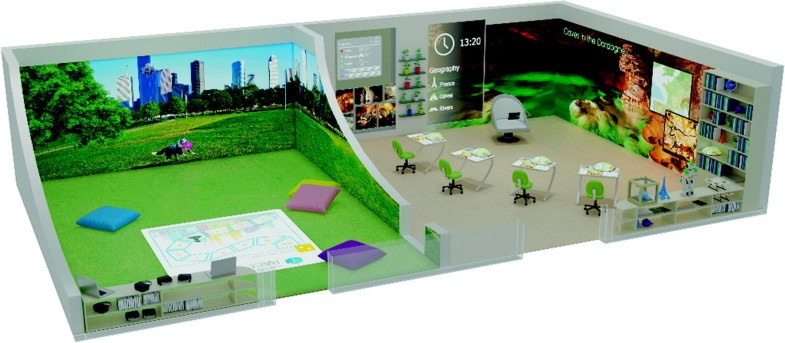
\includegraphics[width=0.55\textwidth]{smart classroom}			
		\caption{智能教室和具有交互功能的墙壁}
		\end{figure}

		而教室墙壁的作用也同样是双重的;一方面,它们将充当交互式智能板,可以展示典型的教育内容(例如,多媒体、笔记、练习),另一方面,他们将能够让学生沉浸在与课程大纲相关的任何环境中(例如,实验室或某地理环境)。而虚拟现实 (VR)、增强现实 (AR) 和 X 现实 (XR) 等最先进的技术将被用来创造极具吸引力和令人难忘的体验。
		
		\subsection{智能教学系统}
		未来的智能教室应该在很大程度上依赖于情景信息,从而做出明智的决定(例如,课程、主题、教学大纲)。因为一个班级由不同的学生组成,他们具有不同的背景、个性、行为、需求和学习模式,因此一个可靠的分析机制将是最重要的,它允许向每个人提供个性化的材料和帮助。
		
		\begin{enumerate}[(1)]
			\item \textbf{智能监测机制}\\作为被动的听众,人们通常发现很难长时间保持恒定的注意力水平,而教学研究表明,在学习中注意力不集中是不可避免的。
				  学生的注意力会从学习转移到其他方面。为此,在教学过程中一种检测注意力不集中行为并选择适当干预措施帮助或支持学生的机制是智能教学系统的基本特征。
			\item \textbf{在线学习资源访问}\\就最终用户应用程序而言,学生应该能够访问一些教育应用程序(例如计算器、字典、多媒体查看器),以及书籍和练习册等。这样,他们将能够 (i) 获得学习的个性化帮助,(ii) 检索有关有趣事物的额外资源(例如,书籍中的一些科普知识),(iii) 可以访问辅助应用程序(例如,计算器、字典等),(iv) 可以访问多媒体,(v) 维护一个可以访问家庭作业历史、电子材料等的个人空间。
			\item \textbf{教师辅助功能}\\智能教学系统能为教师提供专用软件,以支持完整的课堂概览、教学任务的自动化处理和对学生学习情况的智能分析。此外,通过学生学习平台反馈的资料,教师也能轻松掌握各个学生的学习状况,从而给出相应的指导。
		\end{enumerate}

		\begin{figure}[H]
			\centering
			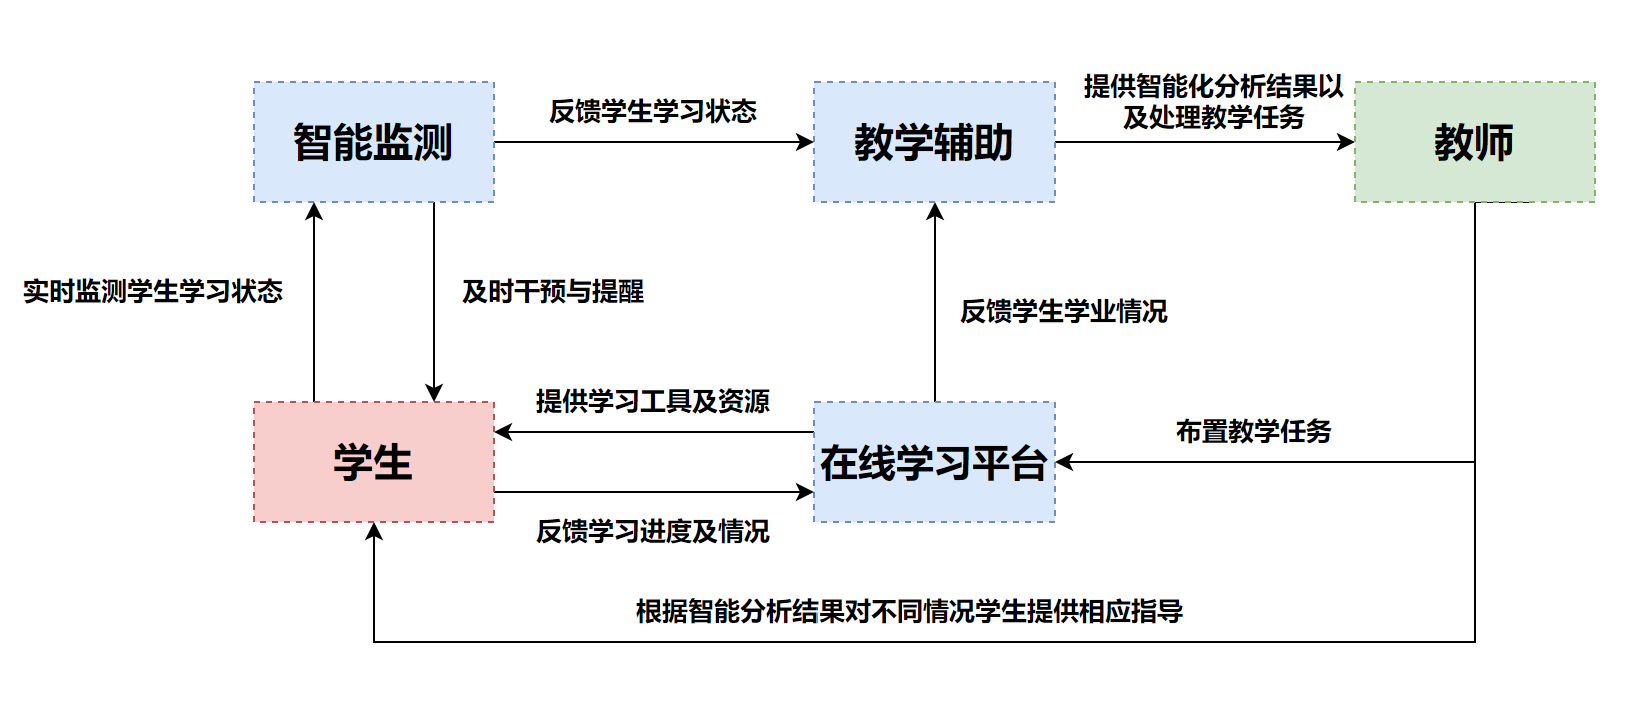
\includegraphics[width=1\textwidth]{fenxi}
			\caption{智能化教学系统}
			\end{figure}
	
	\section{基于大数据的个性化学习实现}
		如何基于基于大数据信息,刻画学习者学习画像,并以此为基础归纳总结出个性化学习路径,提高对学习者的精准指导是目前亟待解决的现实问题。
		我们根据学习者的学习特征及平台学习行为数据为其制定学习画像,在此基础上推送个性化学习路径,优化学习路径指导信息,并在学习过程中根据学习者的学习活动数据分析结果进行个性化学习路径的动态调整,以期帮助学习者完成学习目标。
	\begin{figure}[H]
		\centering
		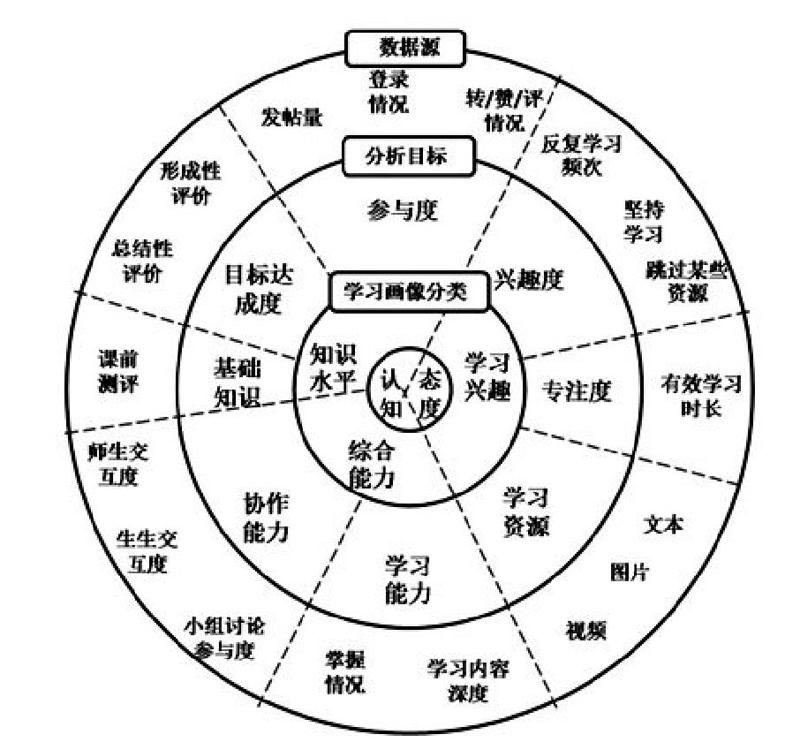
\includegraphics[width=0.5\textwidth]{xuexihuaxiang}
		\caption{学习画像特征模型}
		\end{figure}
		\subsection{学习画像构建}
			\subsubsection{\textbf{数据源的准备分析}}
		数据源主要有静态数据和动态数据两种。静态数据即随着时间的推移相对稳定的数据,主要为用户的基本信息。该类数据的主要来源为:\textcircled{1}学习者基本属性数据,包括学习者的性别、年龄、年级等;\textcircled{2} 学习者学习风格数据。

		动态数据是指在系统应用中随着时间变化而改变的数据,通常能直接反映事物的进程,包括用户的学习行为、浏览行为、访问网站、点击操作等,主要分为以下两类:\textcircled{1}学习者网络行为数据,即学习者在网络环境中集中活跃时间段学习者频繁使用的社交软件,学习者在网络环境中在线或离线学习的表现、连续持续学习时长等,学习者搜索高频词、学习者浏览路径、学习深度、学习完成度、学习者热门收藏网站、评论内容、互动内容等;\textcircled{2}系统反馈数据,即学习平台或任课教师单独提供给学习者关于学习情况的信息数据。
			\subsubsection{\textbf{学习画像框架搭建}}
		在前期学习者基础属性判定与数据收集处理的基础上,经过横向相似性对比、纵向维度划分归纳,结合理论与数据做出如下学习者画像评价指标,其中参与度、兴趣度、专注性、学习深度、抽象能力、协作能力、基础知识、目标达成度等8个为分析目标,知识水平、学习兴趣和综合能力为三个维度。学习者学习画像特征模型如图3所示。
	
	\subsection{基于学习画像的个性化学习路径}
		算法是实现个性化学习路径推荐的关键,目前常用的四种学习路径推荐算法为神经网络、蚁群优化方法、遗传算法以及粒子群算法。经过横纵对比不难发现蚁群算法是一种基于种群寻找最短路径的启发式搜索算法,用来寻找优化路径的概率,具有通用性强、操作简便、求解效率较快等优点。基于此拟采用蚁群算法来实现个性化学习路径的生成与推荐。

		蚁群算法是根据概率转移公式逐步完成求解过程的,其中概率由动态更新的信息素和相对稳定启发信息决定。在本章中我们把学习者学习画像中的特征数据源作为信息素,态度和认知两方面作为启发信息,通过蚁群算法中固定的公式和操作过程,即可完成基于学习画像的个性化学习路径的生成、动态变化、实时分析、个性化推荐,详情如图4所示。
		\begin{figure}[H]
			\centering
			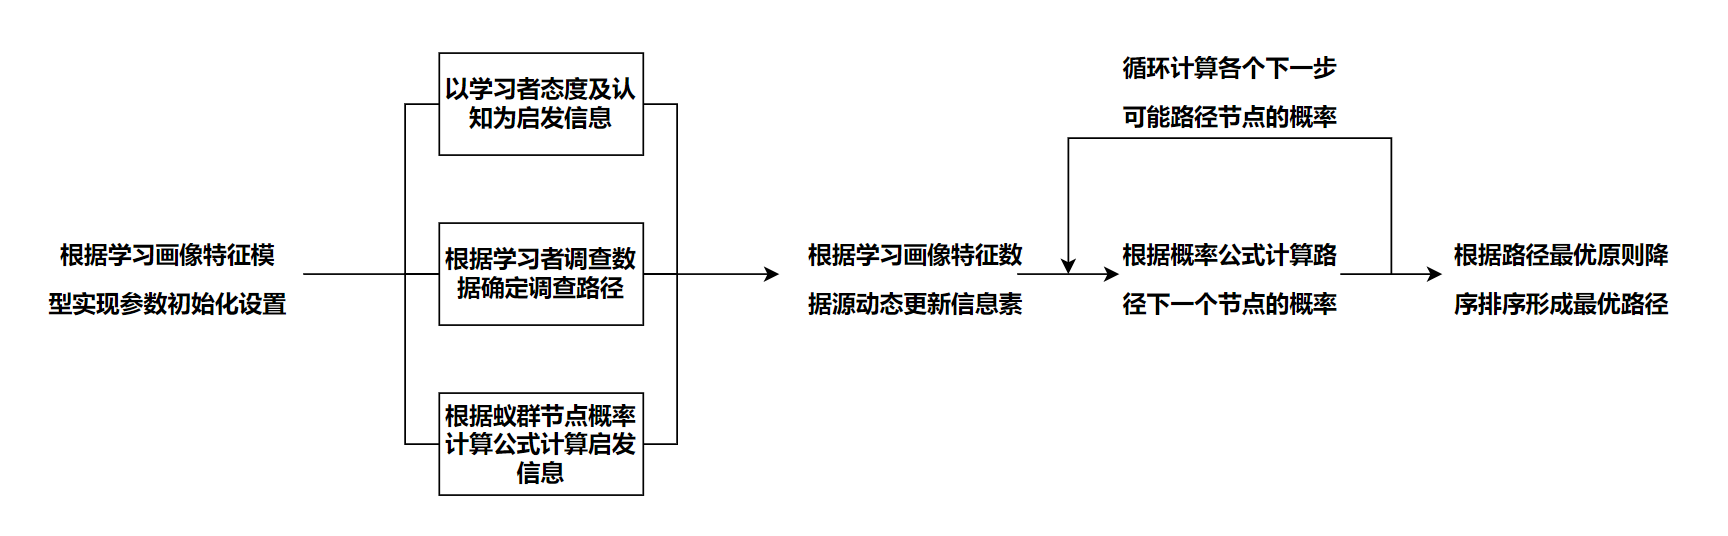
\includegraphics[width=1\textwidth]{yiqun}
			\caption{蚁群算法实现学习路径推荐原理图}
			\end{figure}

	\section{人工智能驱动的虚拟助教}
	人工智能驱动的虚拟助教可以理解为一个旨在改善学生学习体验的程序。许多在线大学课程要求学生需要自学某些知识。但是,当自学量超过老师授课的时间时,结果就不尽如人意了。教师和教授没有足够的时间为每个学生解答疑问或给予帮助。结果,学生花费越来越多的时间尝试在没有帮助的情况下学习。这会产生各种各样的问题,并最终导致学生技能和表现不佳。
	人工智能驱动的虚拟助教可以减轻教师的负担。借助机器学习功能,这些程序不仅可以提供常见问题的答案,还可以分析学习过程并提出优化教育方法的建议。
		\subsubsection{个性化服务}
		作为学生,我们希望在线课程比线下课程更容易。在线学习可以帮助学生设定自己的学习节奏。人工智能驱动的虚拟助教可以为学生提供有关课程、教学方式和难度的充分信息。根据学生以前的学习经验,人工智能驱动的程序还可以为他们的学习速度推荐合适的课程。
		\subsubsection{科学的预测和管理}
		缺乏时间是学生对在线学习不满意的最常见原因之一。他们希望花更少的时间学习,而实际上,他们会花更多的时间,问题在于缺乏有效的时间管理。虚拟助教可以解决时间管理问题。通过设置带有课程和作业提醒的定期日程安排器,虚拟助教可以帮助提醒学生保持进度并提高他们的时间管理技能。
		\subsubsection{及时的支持与鼓励}
		当学生遇到问题时,第一反应是寻求老师的帮助。然而,无论是离线还是在线课堂,一位老师根本没有足够的时间与每个学生交谈。结果,学生没有得到所需的支持并感到孤立。当问题变得复杂时,这样的学生往往会放弃。AI-driver 虚拟助教可以全天候为学生提供支持。借助高质量的应用程序,学生还可以将虚拟助手放在口袋里,从而随时随地获得问题的答案。
		即时支持是学生成功的支柱之一。同时,与程序互动通常会让学生更容易提出所谓的“愚蠢”问题,否则他们会尽量避免这些问题,获得这些问题的答案可以帮助学生更好享受学习的过程。
	
	\section{结语}
	教育部印发的《教育信息化 2.0行动计划》强调:“人工智能、大数据、区块链等技术的迅猛发展,将深刻改变人才需求和教育形态。”将信息技术运用到教学中,不仅体现了科技的进步,也体现了学习方式的变革。未来的教学方式将是“以学为主”的一种学习方式,它不仅表现在获取知识、发展自身能力的方
	面,也是终身教育理论倡导下提升自己竞争力的重要手段。通过提升学生参与感、基于大数据以及人工智能技术实现个性化学习,不仅能够帮助学生更好地适应在线教育方式,还能够提高和增强学生的自主学习能力。
\end{document}